\documentclass[12pt]{article}

\usepackage{fullpage}
\usepackage{multicol,multirow}
\usepackage{tabularx}
\usepackage{ulem}
\usepackage{graphicx}%Вставка картинок правильная
\usepackage{float}%"Плавающие" картинки
\usepackage{wrapfig}%Обтекание фигур (таблиц, картинок и прочего)
\usepackage[utf8]{inputenc}
\usepackage[russian]{babel}

% Оригиналный шаблон: http://k806.ru/dalabs/da-report-template-2012.tex

\begin{document}

\section*{Лабораторная работа №\,7 по курсу дискрeтного анализа: динамическое программирование}

Выполнил студент группы 08-307 МАИ \textit{Дегтярев Денис Андреевич}.

\subsection*{Условие}

Имеется натуральное число n. За один ход с ним можно произвести следующие действия:

 - Вычесть единицу  

 - Разделить на два  
 
 - Разделить на три  

При этом стоимость каждой операции – текущее значение n. Стоимость преобразования - суммарная стоимость всех операций в преобразовании. 
Вам необходимо с помощью последовательностей указанных операций преобразовать число n в единицу таким образом, чтобы стоимость преобразования была наименьшей. 
Делить можно только нацело.

\subsection*{Метод решения}

Данную задачу решал с помощью динамического программирования.

\subsection*{Описание программы}

Создаем массив для dp, туда записываем минимальные суммы, требуемые, чтобы туда попасть и операция, которую нужно выполнить, чтобы туда попасть.
Далее по backtrackingу просто восстанавливаем путь от 1 до n.

\subsection*{Дневник отладки}  
  
 
    - Сначала ML - моя структура содержала путь от n до любого из элементов - много памяти, при n = $10^7$, поэтому оставил только одну операцию.

    - Затем WA, посчитал максимальную val, по арифметической прогрессии оно может быть равно ($10^7$+1) * $10^7$ \approx $10^{14}$ (long long), а у меня было int ($10^9$).  

\subsection*{Тест производительности}

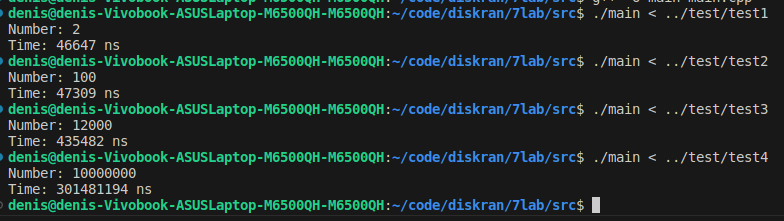
\includegraphics[width=7in]{time.png}

\subsection*{Недочёты}

Недочетов не должно быть... Реализовывал все добросовестно.

\subsection*{Выводы}

Выполнив лабораторную работу №7 по курсу «Дискретный анализ», я изучил
динамическое программирование и убедился, что оно помогает в оптимизации
решения задачи, благодаря разбиению задачи и решению более простых
подзадач.

\end{document}
